\subsection{Sample-size-dependent populations}\label{sec:reslocal}

\begin{figure}[t]
\centering
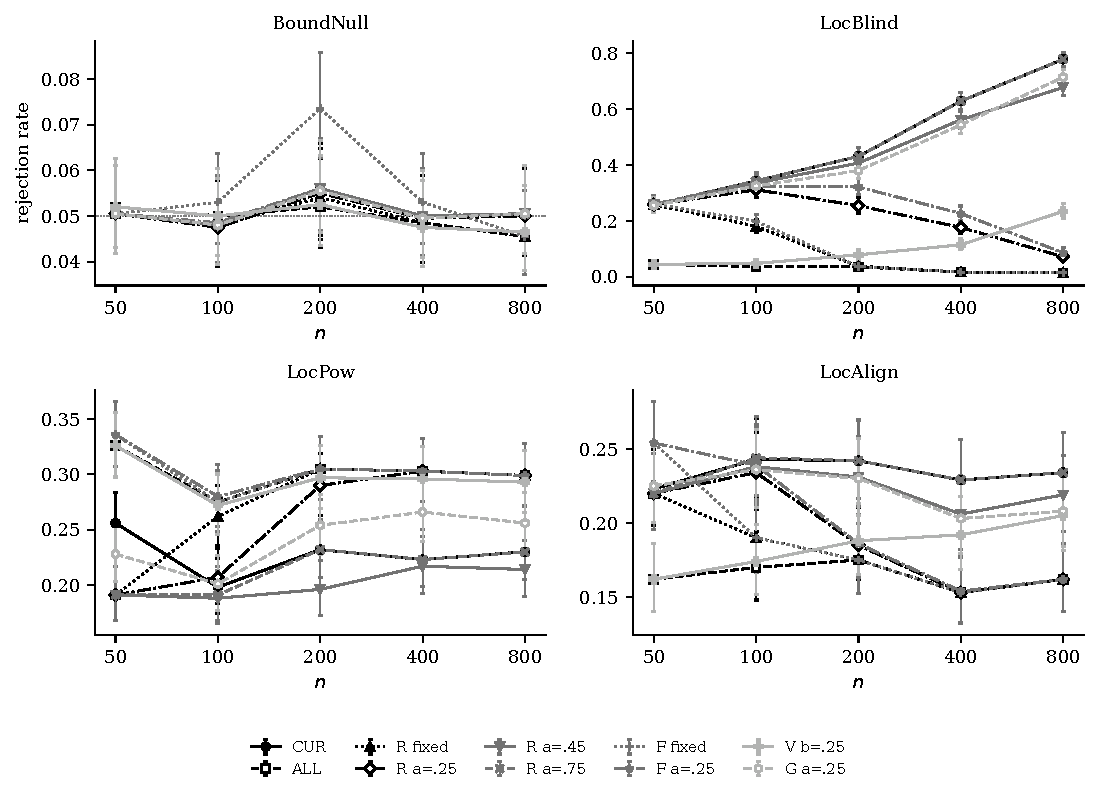
\includegraphics[width=\textwidth]{gen/fig_B_local.pdf}
\caption{B\_local: rejection rates against $n$ when the populations change with $n$ (Wilson 95\% intervals; dotted line at $0.05$ in BoundNull). The radius schedule used to construct BoundNull and LocBlind is $\theta_n^{(0.25)}$. Full table in \cref{tab:Blocal}.}\label{fig:Blocal}
\end{figure}

\paragraph{The local blind spot (LocBlind).} This is the sequence of \cref{thm:localblind} with $c=1/2$. Current-only power rises from $0.255$ to $0.779$ between $n=50$ and $n=800$, since $\sqrt n\,D(Q_c,Q_{t,n})$ grows like $n^{1/4}$. R-$\theta^{(0.25)}$ follows it at first and then turns down: $0.311$, $0.254$, $0.176$ and $0.071$ at $n=100,\dots,800$. Over the same range its acceptance rate in the observed row rises from $0.36$ to $0.93$. The fixed radius fails earlier ($0.013$ at $n=800$), and so does ALL. The frozen F-$\theta^{(0.25)}$ and PB-$\theta^{(0.25)}$ behave like R-$\theta^{(0.25)}$ ($0.085$ and $0.072$ at $n=800$). The safeguard keeps most of the current-only power ($0.715$). The faster schedules ($a=0.45,0.75$) escape this particular sequence only because their radius falls below $D(Q_c,Q_{h,n})=\theta^{(0.25)}_n/2$, so they reject the source. A sequence built at their own radius would trap them in the same way. Vanishing masses recover slowly ($0.234$ and $0.580$ at $n=800$).

\paragraph{Identical source, $\sqrt n$-local alternative (LocPow).} Retaining the identical source pays off here. For $n\ge200$, R-$\theta^{\rm fix}$ and R-$\theta^{(0.25)}$ reject at $0.29$--$0.31$ against $0.22$--$0.23$ for current-only testing, close to ALL (always pooling, which is optimal here). With $a=0.75$ the source is discarded (acceptance $0.017$ at $n=200$), and the test coincides with current-only testing. The intermediate $a=0.45$ retains the source in $81$--$92\%$ of data sets but gains nothing; its rate ($0.19$--$0.22$) is even slightly below current-only testing. In reselected rows a source that is accepted only sometimes adds noise to the reference distribution. At $n=50$, all reselected radius tests are below current-only testing ($0.191$ vs.\ $0.256$), while frozen tests are above it ($0.336$); the frozen numbers are not comparable, because of size distortion at small $n$ (\cref{tab:Bnull}). Vanishing masses ($0.27$--$0.30$) retain most of the gain over this range of $n$. This is consistent with \cref{prop:nogain}, which is asymptotic: $b_n^{(0.25)}$ is still $0.33$ at $n=800$.

\paragraph{Shift aligned with the effect (LocAlign).} When the historical source is shifted by $2/\sqrt n$ in the direction of a $2.5/\sqrt n$ effect, every procedure that keeps the source loses power ($0.15$--$0.18$ against $0.23$). This includes R-$\theta^{(0.25)}$ for $n\ge400$, because a $\sqrt n$-local shift is always inside a radius $\gg n^{-1/2}$. The original partial bootstrap drops to $0.047$--$0.060$, which is essentially no power. R-$\theta^{(0.45)}$ ($0.21$--$0.23$) and the safeguard ($0.20$--$0.24$) lose little. This is the $\sqrt n$-scale version of the trade-off in \cref{cor:tradeoff}: a radius large enough to retain an identical source cannot distinguish it from a source shifted at the sampling scale.

\paragraph{Boundary null (BoundNull).} With the source exactly at distance $\theta^{(0.25)}_n$, every reselected and fixed-rule test stays at $0.045$--$0.056$. The $a=0.25$ schedule almost never accepts the source (acceptance $\le0.002$), since $\hat D+q$ exceeds $\theta_n$ whenever $\hat D\approx\theta_n$. The informative cell is the fixed radius. There the same source sits well inside $\theta=0.5$ for large $n$, and its acceptance probability passes through intermediate values ($0.36$ at $n=200$). In that cell the frozen test F-$\theta^{\rm fix}$ rejects at $0.073$ (interval above $0.05$), while the reselected test gives $0.054$. This is the predicted non-uniformity of frozen calibration: inflation appears exactly where the selection probability is neither near $0$ nor near $1$.
